\documentclass[12pt,a4paper]{article}
\usepackage[spanish,es-nodecimaldot]{babel}
\usepackage[utf8]{inputenc}
\usepackage[T1]{fontenc}
\usepackage{lmodern}
\usepackage{geometry}
\geometry{margin=2.5cm}
\usepackage{microtype,graphicx,booktabs,longtable,array,enumitem,xcolor,listings,tikz,hyperref,cleveref,fancyhdr,float}
\usetikzlibrary{arrows.meta,positioning,shapes.geometric}
\hypersetup{colorlinks=true,linkcolor=blue!45!black,urlcolor=blue!55!black,citecolor=blue!45!black,pdftitle={Análisis de patrones de cobertura periodística en La República},pdfauthor={Grupo 3 -- DS3021}}
\pagestyle{fancy}\fancyhf{}\lhead{DS3021 -- Análisis Computacional de Datos}\rhead{Proyecto final -- Parte II}\cfoot{\thepage}
\setlength{\headheight}{14.5pt}
\setlength{\parskip}{0.45em}\setlength{\parindent}{0pt}
\setlist[itemize]{topsep=3pt,itemsep=2pt}\setlist[enumerate]{topsep=3pt,itemsep=2pt}
\lstset{basicstyle=\ttfamily\small,keywordstyle=\color{blue!65!black}\bfseries,commentstyle=\color{green!40!black},stringstyle=\color{red!55!black},showstringspaces=false,breaklines=true,frame=single,rulecolor=\color{black!20},columns=fullflexible,keepspaces=true}
% Rutas y nombres de archivo largos: permite cortar la línea en / _ . -
\makeatletter\g@addto@macro\UrlBreaks{\do\_\do\-}\makeatother
\begin{document}

\begin{titlepage}
    \thispagestyle{empty}
    \begin{center}

        {\large\bfseries UNIVERSIDAD DE INGENIERÍA Y TECNOLOGÍA\par}

        \vspace{0.5cm}

        
\includegraphics[width=3.6cm]{UTEC-Logo.jpg}

        \vspace{0.5cm}

        {\bfseries FACULTAD DE COMPUTACIÓN\par}

        \vspace{0.15cm}

        {\bfseries CARRERA DE DATA SCIENCE\par}

        \vspace{0.7cm}

        {\bfseries SEGUNDO AVANCE DEL PROYECTO FINAL:\par}

        \vspace{0.3cm}

        {\Large\bfseries
        Análisis de patrones de cobertura periodística\\
        en La República
        \par}

        \vspace{0.7cm}

        {\bfseries CURSO:\par}

        \vspace{0.15cm}

        {\bfseries ANÁLISIS COMPUTACIONAL DE DATOS (DS3021)\par}

        \vspace{0.1cm}

        {\small Semestre 2026-1\par}

        \vspace{0.6cm}

        {\bfseries ESTUDIANTES:\par}

        \vspace{0.25cm}

        {\small
        Aguirre Milla, Fernando\par
        \vspace{0.15cm}
        Toribio Arrieta, Josue Raul\par
        \vspace{0.15cm}
        Hurtado Vite, Mia Dayhana\par
        \vspace{0.15cm}
        Pacheco Vera, Fatima Isabella\par
        \vspace{0.15cm}
        Romano Castro, Aaron Adriano\par
        }

        \vfill

        {\bfseries LIMA -- PERÚ\par}

        \vspace{0.1cm}

        {\bfseries 2026\par}

        \vspace{0.3cm}

        {\small Repositorio: \url{https://github.com/josueTori-UTEC/ACD-Analisis-Noticias-LaRepublica}\par}

    \end{center}
\end{titlepage}

\setcounter{page}{1}
\begin{abstract}
Se trabajó con 1\,116 noticias de La República recopiladas por scraping en la Parte I. Se construyó un pipeline reproducible que limpia, integra, reduce y transforma los datos hasta un dataset de 31 variables, y se analizó cómo se distribuyen las noticias por sección, autor, hora, fecha y características del titular.

Los resultados principales son tres. Primero, la muestra está muy sesgada hacia el tiempo del scraping: el \textbf{43,4\,\%} de las noticias es de agosto y septiembre de 2026, y la composición por sección cambia mucho de un año a otro (V de Cramér = 0,61). Segundo, \texttt{fecha} es siempre igual o posterior a la fecha escrita en la URL, difiere en el \textbf{38,4\,\%} de los casos y llega a 1\,632 días de diferencia, por lo que probablemente no sea siempre la fecha de publicación. Tercero, el estilo del titular (cifras, comillas, preguntas) y el horario dependen del área editorial, con tamaños de efecto moderados.
\end{abstract}
\newpage
\tableofcontents
\newpage

% =====================================================================
\section{Identificación}
\textbf{Título:} Análisis de patrones de cobertura periodística en La República. \textbf{Unidad de análisis:} una noticia identificada por su URL. \textbf{Fuente:} páginas públicas de \href{https://larepublica.pe}{larepublica.pe}, obtenidas por scraping en la Parte I \cite{larepublica}.

\begin{table}[H]\centering
\caption{Integrantes y responsabilidades en la Parte II.}
\begin{tabular}{p{5.2cm}p{9.6cm}}
\toprule
\textbf{Integrante} & \textbf{Responsabilidad en la Parte II}\\\midrule
Aguirre Milla, Fernando & Coordinación general, ingesta y descripción del origen de los datos (Parte I)\\
Toribio Arrieta, Josue Raul & Integración de metadatos y construcción de la base analítica (notebook 01)\\
Hurtado Vite, Mia Dayhana & Validaciones de calidad y pruebas estadísticas\\
Pacheco Vera, Fatima Isabella & Diccionario de datos, README y reproducibilidad del repositorio\\
Romano Castro, Aaron Adriano & Análisis visual, interpretación, redacción del informe y presentación\\
\bottomrule
\end{tabular}
\end{table}

% =====================================================================
\section{Contexto actualizado}
Un diario digital publica cientos de notas por semana repartidas en decenas de secciones, etiquetas y firmas. Navegando el portal es difícil ver cómo se compone esa producción. El análisis de datos permite resumirla: qué secciones pesan más, cuánto se concentran los autores, a qué horas se publica y cómo se redactan los titulares.

En la Parte I se recopilaron 1\,116 noticias con siete variables (etiqueta, titular, longitud, URL, autor, hora y fecha) para fechas entre el 31 de octubre de 2022 y el 22 de septiembre de 2026. Al revisar el material en la Parte II aparecieron tres condiciones que reorientaron el problema:
\begin{itemize}
\item \textbf{La muestra no es aleatoria ni continua.} Cubre 416 fechas distintas, y el 43,4\,\% de las noticias es de agosto y septiembre de 2026. Por eso no se puede estimar el peso real de una sección en el diario; sí se puede describir esta colección y medir su sesgo.
\item \textbf{La fecha es ambigua.} En 428 de las 1\,115 URL que incluyen fecha, esta no coincide con el campo \texttt{fecha}.
\item \textbf{No hay texto de la noticia ni métricas de lectura.} El análisis se limita a metadatos y titulares.
\end{itemize}
Por eso el problema se acotó a \textbf{caracterizar la colección y evaluar su calidad y sus sesgos}, de modo que cualquier equipo que la reutilice sepa qué puede y qué no puede concluir de ella.

% =====================================================================
\section{Objetivos actualizados}
\textbf{Objetivo general:} caracterizar los patrones de cobertura que se observan en la colección de noticias de La República y documentar los sesgos de la muestra mediante un proceso reproducible de preparación, análisis y visualización de datos.

\textbf{Objetivos específicos:}
\begin{itemize}
\item Medir el sesgo temporal y de rutas de la muestra, y su efecto sobre la composición por sección.
\item Evaluar la confiabilidad de \texttt{fecha} y \texttt{hora} y detectar anomalías.
\item Describir la concentración de autores y etiquetas y su relación con las secciones.
\item Comparar los titulares (longitud, cifras, preguntas, comillas) entre áreas editoriales con pruebas estadísticas.
\item Entregar un dataset documentado, un pipeline ejecutable y recomendaciones para quien reutilice la colección.
\end{itemize}
Los objetivos de la Parte I, más amplios, hablaban de describir la cobertura periodística del diario. Se reformularon porque los datos permiten describir la colección, no la producción total del medio.

% =====================================================================
\section{Dataset y diccionario de datos final}
El archivo \path{data/noticias_larepublica_final.csv} conserva las 1\,116 filas y amplía el esquema de 7 a 31 variables. También se guarda en una base SQLite (\path{data/noticias_larepublica.db}). El diccionario completo está en \path{docs/Diccionario_de_datos_final.pdf}.

\begin{table}[H]\centering
\caption{Indicadores generales del dataset final.}
\begin{tabular}{p{7cm}p{7.5cm}}
\toprule
\textbf{Indicador} & \textbf{Valor}\\\midrule
Registros & 1\,116\\
Variables originales / finales & 7 / 31\\
URL únicas & 1\,116 (0 duplicadas)\\
Rango de fechas & 31-10-2022 a 22-09-2026 (416 fechas distintas)\\
Secciones (originales / agrupadas) & 28 / 13\\
Etiquetas (originales / agrupadas) & 408 / 54\\
Autores distintos & 121\\
Valores faltantes finales & 2 (\texttt{fecha\_url} y \texttt{dias\_desfase} de una misma noticia)\\
\bottomrule
\end{tabular}
\end{table}

\textbf{Limitaciones del dataset.}
\begin{enumerate}
\item Muestra no probabilística, concentrada en agosto y septiembre de 2026.
\item \texttt{fecha} puede no ser la fecha de publicación.
\item Hay 37 horas exactamente en 00:00 o 05:00, probablemente programadas.
\item \texttt{seccion} viene de la URL y \texttt{area\_editorial} de un catálogo propio del grupo, por lo que no son clasificaciones oficiales.
\item No hay texto completo, audiencia ni historial de actualización.
\end{enumerate}

% =====================================================================
\subsection{Diccionario de datos final}
La tabla describe las 31 variables con el formato del diccionario del curso. El tamaño máximo es la mayor cantidad de caracteres que ocupa un valor en el CSV final. Las variables booleanas se guardan como \texttt{True} o \texttt{False}.

{\footnotesize\setlength{\tabcolsep}{3pt}\setlength{\LTcapwidth}{\textwidth}
\begin{longtable}{>{\raggedright\arraybackslash}p{3.6cm}>{\raggedright\arraybackslash}p{3.3cm}>{\raggedright\arraybackslash}p{1.7cm}>{\centering\arraybackslash}p{1.4cm}>{\raggedright\arraybackslash}p{2.6cm}>{\centering\arraybackslash}p{1.7cm}}
\caption{Diccionario de datos final (\texttt{noticias\_larepublica\_final.csv}).}\label{tab:diccionario}\\
\toprule
\textbf{Variable} & \textbf{Descripción} & \textbf{Tipo} & \textbf{Tamaño máximo} & \textbf{Valores} & \textbf{Unidad}\\\midrule
\endfirsthead
\toprule
\textbf{Variable} & \textbf{Descripción} & \textbf{Tipo} & \textbf{Tamaño máximo} & \textbf{Valores} & \textbf{Unidad}\\\midrule
\endhead
\texttt{tag} & Etiqueta temática de la noticia; las 10 ausentes se codifican «Sin etiqueta» & Categórico & 48 & JNE, Dólar, Sin etiqueta, \dots{} (408 valores) & -\\
\texttt{tag\_agrupado} & Etiqueta con 5 o más noticias; el resto pasa a «Otras etiquetas» & Categórico & 31 & Impresa, Otras etiquetas, \dots{} (54 valores) & -\\
\texttt{titulo} & Titular completo, normalizado (Unicode NFC y espacios simples) & Texto & 191 & Texto libre & -\\
\texttt{longitud\_titulo} & Cantidad de caracteres del titular, recalculada desde titulo & Numérico & 3 & 33 a 191 & Caracteres\\
\texttt{rango\_longitud} & Tercil de la longitud del titular & Categórico & 5 & Corto (33--95), Medio (96--110), Largo (111--191) & -\\
\texttt{palabras\_titulo} & Cantidad de palabras del titular & Numérico & 2 & 5 a 32 & Palabras\\
\texttt{contiene\_pregunta} & Indica si el titular tiene ¿ o ? & Booleano & 5 & True, False & -\\
\texttt{contiene\_cifra} & Indica si el titular tiene al menos un dígito & Booleano & 5 & True, False & -\\
\texttt{contiene\_dos\_puntos} & Indica si el titular tiene «:» & Booleano & 5 & True, False & -\\
\texttt{contiene\_comillas} & Indica si el titular tiene comillas (rectas, tipográficas o angulares) & Booleano & 5 & True, False & -\\
\texttt{url} & Enlace de la noticia; identificador único del registro & Texto & 273 & \url{https://larepublica.pe/}\dots{} & -\\
\texttt{url\_hnews} & Indica si la URL tiene el marcador «hnews» (formato de URL desde 2025) & Booleano & 5 & True, False & -\\
\texttt{seccion} & Sección del portal, tomada del primer segmento de la URL & Categórico & 18 & Mundo, Política, Economía, \dots{} (28 valores) & -\\
\texttt{seccion\_agrupada} & Sección con 20 o más noticias; el resto pasa a «Otras secciones» & Categórico & 16 & Mundo, Otras secciones, \dots{} (13 valores) & -\\
\texttt{area\_editorial} & Área editorial según el catálogo del grupo & Categórico & 25 & Actualidad, Internacional, Entretenimiento y cultura, Deportes, Ciencia y tecnología, Servicios y comerciales & -\\
\texttt{autor} & Firma de la noticia (incluye firmas institucionales) & Categórico & 25 & Judith Sequeiros, Redacción LR, \dots{} (121 valores) & -\\
\texttt{autor\_institucional} & Indica si la firma es institucional (Redacción LR o agencia) & Booleano & 5 & True, False & -\\
\texttt{fecha} & Fecha registrada en la noticia; puede ser de actualización & Fecha & 10 & 2022-10-31 a 2026-09-22 & AAAA-MM-DD\\
\texttt{fecha\_url} & Fecha escrita en la ruta de la URL (1 vacío) & Fecha & 10 & 2021-12-08 a 2026-09-22 & AAAA-MM-DD\\
\texttt{dias\_desfase} & Días entre fecha y fecha\_url; nunca negativo (1 vacío) & Numérico & 4 & 0 a 1632 & Días\\
\texttt{desfase\_cat} & Categoría del desfase & Categórico & 16 & Mismo día, 1 a 7 días, Más de 7 días, Sin fecha en URL & -\\
\texttt{anio} & Año de fecha & Numérico & 4 & 2022 a 2026 & Año\\
\texttt{mes} & Mes de fecha & Numérico & 2 & 1 a 12 & Mes\\
\texttt{anio\_mes} & Año y mes de fecha & Texto & 7 & 2022-10 a 2026-09 (39 valores) & AAAA-MM\\
\texttt{periodo\_muestra} & Marca si la fecha cae en agosto-septiembre de 2026 & Categórico & 19 & Ago-Sep 2026, Anterior a ago 2026 & -\\
\texttt{dia\_semana} & Día de la semana de fecha & Categórico & 9 & Lunes a Domingo & -\\
\texttt{fin\_de\_semana} & Indica si fecha cae en sábado o domingo & Booleano & 5 & True, False & -\\
\texttt{hora} & Hora registrada, normalizada a HH:MM & Hora & 5 & 00:00 a 23:59 & HH:MM\\
\texttt{hora\_num} & Hora entera extraída de hora & Numérico & 2 & 0 a 23 & Horas\\
\texttt{franja\_horaria} & Tramo del día según hora\_num & Categórico & 17 & Madrugada (00-05), Mañana (06-11), Tarde (12-17), Noche (18-23) & -\\
\texttt{hora\_sospechosa} & Indica si hora es exactamente 00:00 o 05:00 & Booleano & 5 & True, False & -\\
\bottomrule
\end{longtable}
}

% =====================================================================
\section{Propuesta de pipeline}
El pipeline parte de un CSV congelado de la Parte I, de modo que el resultado no dependa de que el sitio web mantenga su HTML. Tiene seis etapas, que se ejecutan con \texttt{python run\_all.py}:

\begin{figure}[H]\centering
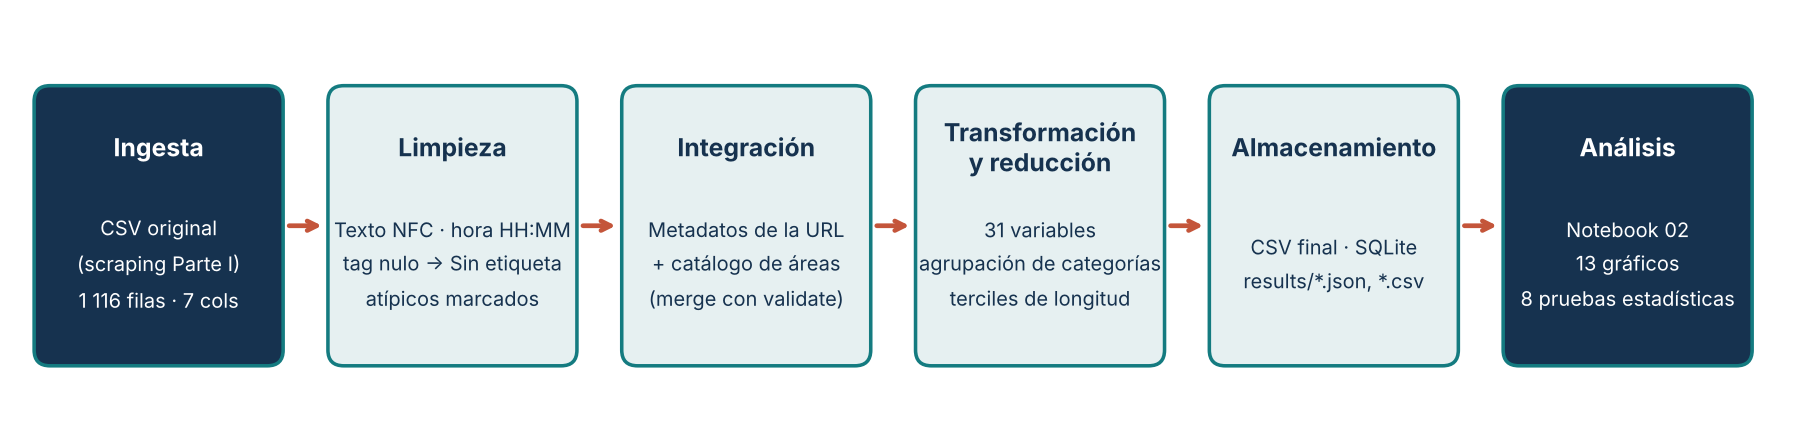
\includegraphics[width=\textwidth]{figures/14_pipeline.png}
\caption{Flujo de datos del proyecto.}
\label{fig:pipeline}
\end{figure}

\begin{table}[H]\centering
\caption{Etapas del pipeline y dónde se implementa cada una.}
\begin{tabular}{p{3.2cm}p{7.5cm}p{3.5cm}}
\toprule
\textbf{Etapa} & \textbf{Qué hace} & \textbf{Dónde}\\\midrule
Ingesta & Lee \path{data/noticias_larepublica_original.csv} y valida que tenga las 7 columnas esperadas. El CSV es la salida del scraping de la Parte I. & Notebook 01, secciones 1 y 2\\
Limpieza & Normaliza texto y hora, trata faltantes y marca atípicos y horas sospechosas. & Notebook 01, sección 2\\
Integración & Une metadatos de la URL (sección, fecha, marcador \texttt{hnews}) y un catálogo de áreas editoriales, con \texttt{merge(validate=...)}. & Notebook 01, sección 3\\
Transformación y reducción & Crea 24 variables y agrupa categorías raras. & Notebook 01, secciones 4 y 5\\
Almacenamiento & Escribe el CSV final, la base SQLite y los resultados (\path{results/}). & Notebook 01, secciones 6 y 8\\
Análisis & Genera 13 gráficos y una tabla de 8 pruebas estadísticas. & Notebook 02\\
\bottomrule
\end{tabular}
\end{table}

\textbf{Decisiones de diseño.} Se usaron CSV y SQLite en lugar de un servidor de base de datos porque el volumen (1\,116 filas, 0,5 MB) no lo justifica y ambos formatos son portables. SQLite permite consultar con SQL, por ejemplo agrupar por área editorial. Cada etapa termina con validaciones automáticas (\texttt{assert}) que detienen el notebook si se pierden filas, hay URL repetidas o aparecen desfases negativos. Una actualización de datos solo requiere reemplazar el CSV de entrada y ejecutar de nuevo. El scraper de la Parte I queda fuera de este repositorio y no se vuelve a ejecutar.

% =====================================================================
\section{Preprocesamiento de datos}
Antes de aplicar cada tratamiento se midió el problema (notebook 01, sección 2.1). El resultado fue el siguiente:

{\small
\begin{longtable}{p{2.3cm}p{3.9cm}p{5.4cm}p{2.6cm}}
\caption{Problemas observados y tratamiento aplicado en el preprocesamiento.}\\
\toprule
\textbf{Actividad} & \textbf{Problema observado} & \textbf{Decisión y justificación} & \textbf{Resultado}\\\midrule
\endfirsthead
\toprule
\textbf{Actividad} & \textbf{Problema observado} & \textbf{Decisión y justificación} & \textbf{Resultado}\\\midrule
\endhead
Estructura & Se esperaban 7 columnas & Validación con \texttt{assert}; si falla, se detiene & 7 columnas\\
Duplicados & Se buscó por \texttt{url} y por \texttt{titulo} & La URL es el identificador; el titular solo no basta & 0 duplicados\\
Faltantes & 10 \texttt{tag} vacíos, en 6 secciones distintas & Se codifican «Sin etiqueta». Imputar un tema no tiene base, y borrar las filas perdería noticias con el resto de campos completos & 10 registros\\
Texto & 23 longitudes distintas al texto; 8 titulares con espacios sobrantes & Normalización Unicode NFC y espacios simples; longitud recalculada & 31 longitudes corregidas\\
Hora & 245 horas sin cero inicial (5:00) & Formato HH:MM; evita errores de orden y de extracción & 245 normalizadas\\
Atípicos & Regla 1,5\,×\,IQR sobre la longitud (Q1 = 90,75; Q3 = 115; límites 54,38 y 151,38) & Se usa como detector. Los casos revisados son titulares reales (notas breves o con declaraciones); se conservan & 40 (29 cortos, 11 largos)\\
Horas sospechosas & 21 noticias a las 05:00 y 16 a las 00:00, frente a unas 5 por hora entre 01 y 04 & Se conservan y se marcan con \texttt{hora\_sospechosa}. De las 16 de medianoche, 13 son horóscopos programados & 37 marcadas\\
Integración & La sección y la fecha están dentro de la URL & Tabla auxiliar de metadatos y catálogo de áreas, con \texttt{validate='one\_to\_one'} y \texttt{'many\_to\_one'} & 28 secciones, 6 áreas\\
Reducción & Alta cardinalidad: 28 secciones y 408 etiquetas (251 aparecen una vez) & Agrupar secciones con menos de 20 noticias y etiquetas con menos de 5. Se conservan las columnas originales & Secciones 28\,$\to$\,13; etiquetas 408\,$\to$\,54\\
Discretización & Longitud continua (33--191) & Terciles con \texttt{pd.qcut}: grupos de tamaño parejo para comparar & Corto $\le$\,95 · Medio 96--110 · Largo $\ge$\,111\\
\bottomrule
\end{longtable}
}

\textbf{Sobre los faltantes.} Con 10 casos no hay potencia para una prueba formal de mecanismo, pero se verificó que no se concentran en una sola ruta: están repartidos en seis secciones, lo que descarta un fallo del scraping en un solo punto. Por eso se tratan como ausencia de etiqueta y no como error de captura.

\textbf{Sobre la integración.} La integración usa dos fuentes: los metadatos que se leen en la URL y un catálogo de secciones elaborado por el grupo. No se integraron bases externas porque no existe otra fuente que se pueda enlazar por noticia sin texto completo.

% =====================================================================
\section{Feature engineering}
Se crearon 24 variables a partir de las 7 originales. Se agruparon por la pregunta que ayudan a responder y se verificó que cada una se use en el análisis.

{\small
\begin{longtable}{p{4.1cm}p{4.2cm}p{3.3cm}p{2.5cm}}
\caption{Variables derivadas, cómo se construyen y dónde se usan.}\\
\toprule
\textbf{Variables} & \textbf{Construcción} & \textbf{Para qué sirven} & \textbf{Se usa en}\\\midrule
\endfirsthead
\toprule
\textbf{Variables} & \textbf{Construcción} & \textbf{Para qué sirven} & \textbf{Se usa en}\\\midrule
\endhead
\texttt{periodo\_muestra}, \texttt{anio}, \texttt{mes}, \texttt{anio\_mes} & Componentes de fecha; marca si cae en ago-sep 2026 & Medir el sesgo temporal & Figuras \ref{fig:mes} y \ref{fig:seccion-anio}\\
\texttt{fecha\_url}, \texttt{dias\_desfase}, \texttt{desfase\_cat} & Fecha en la ruta de la URL y diferencia en días con \texttt{fecha} & Evaluar la confiabilidad de \texttt{fecha} & Figura \ref{fig:desfase}\\
\texttt{hora\_num}, \texttt{franja\_horaria}, \texttt{hora\_sospechosa} & Hora entera, tramos de 6 horas, 00:00 o 05:00 exactas & Horarios y anomalías & Figuras \ref{fig:horas} y \ref{fig:franja}\\
\texttt{dia\_semana}, \texttt{fin\_de\_semana} & Derivadas de \texttt{fecha} & Efecto del día & Figura \ref{fig:dias}\\
\texttt{seccion}, \texttt{seccion\_agrupada}, \texttt{area\_editorial} & Primer segmento de la URL; agrupación; catálogo de 6 áreas & Comparar grupos de tamaño suficiente & Figuras \ref{fig:secciones}, \ref{fig:seccion-anio}, \ref{fig:longitud} a \ref{fig:franja}\\
\texttt{tag\_agrupado} & Etiquetas con 5 o más noticias & Reducir la cola larga & Figura \ref{fig:etiquetas}\\
\texttt{palabras\_titulo}, \texttt{rango\_longitud} & Conteo de palabras; terciles de longitud & Describir la extensión & Figura \ref{fig:longitud}\\
\texttt{contiene\_pregunta}, \texttt{\_cifra}, \texttt{\_dos\_puntos}, \texttt{\_comillas} & Expresiones regulares sobre el titular & Comparar estilo de redacción & Figura \ref{fig:rasgos}\\
\texttt{autor\_institucional} & Firma «Redacción LR» o de agencia & Separar firmas no personales & Sección \ref{sec:autores}\\
\texttt{url\_hnews} & Marcador \texttt{hnews} en la URL & Detectar un cambio de formato & Figura \ref{fig:hnews}\\
\bottomrule
\end{longtable}
}

Tres de estas variables cambiaron los hallazgos. \texttt{dias\_desfase} permitió descubrir la cola de hasta 1\,632 días. \texttt{hora\_sospechosa} mostró que el pico de madrugada era en buena parte artificial. \texttt{url\_hnews} reveló que el formato de las URL cambió en 2025. Ninguna de las tres existía en el dataset original.

% =====================================================================
\section{Análisis y visualización de datos}
El análisis combina frecuencias, tablas cruzadas y pruebas de hipótesis. Como la muestra no es aleatoria, los valores $p$ describen asociaciones dentro de esta colección y no se extrapolan al diario. Se reportan tamaños de efecto, porque con 1\,116 observaciones casi cualquier diferencia sale significativa.

\subsection{Composición de la muestra y sesgo temporal}
\begin{figure}[H]\centering
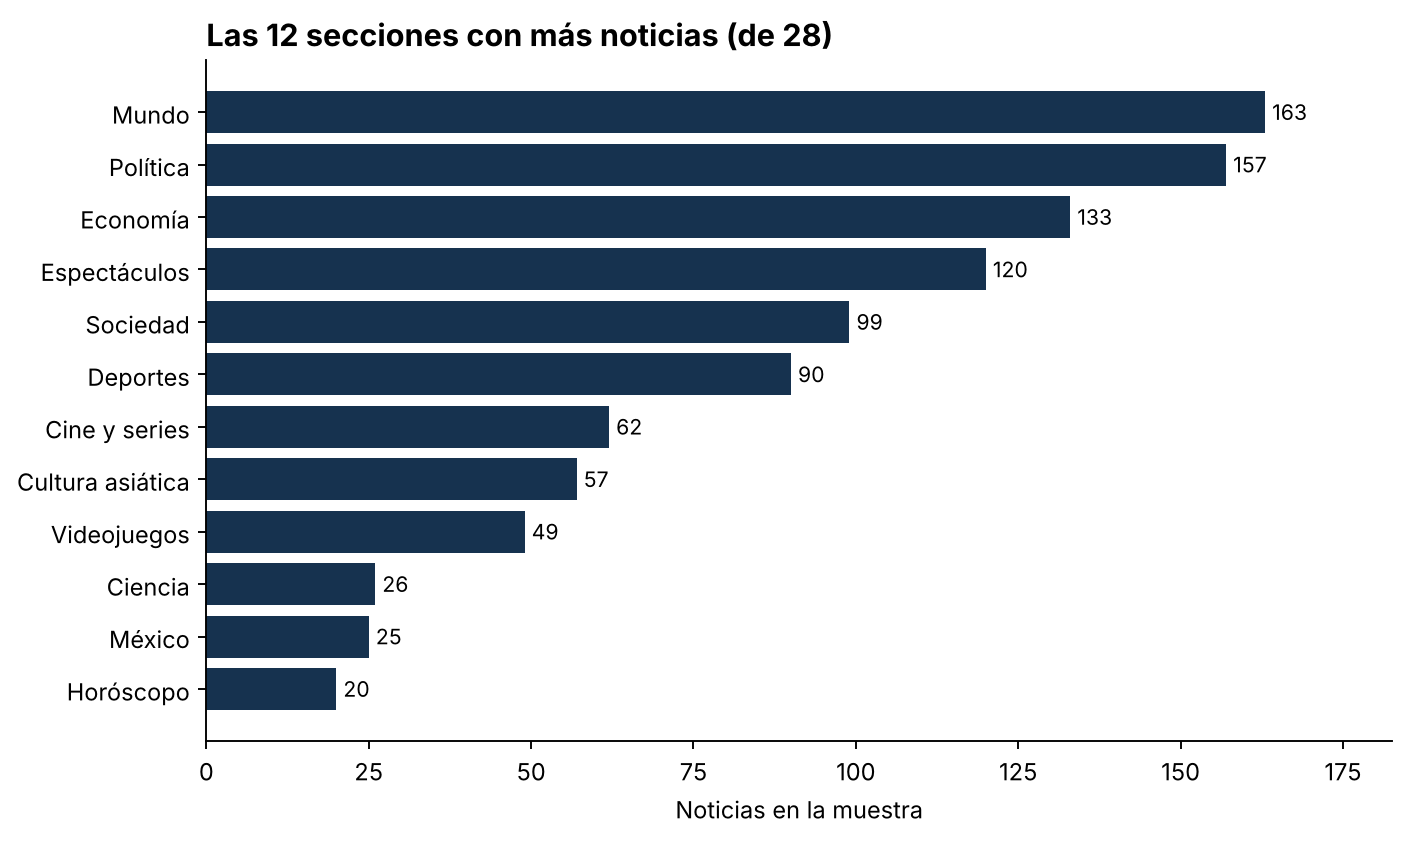
\includegraphics[width=0.85\textwidth]{figures/01_secciones.png}
\caption{Las 12 secciones con más noticias.}
\label{fig:secciones}
\end{figure}
Mundo (163), Política (157) y Economía (133) lideran, y seis secciones suman el 68,28\,\%. Esta composición depende de cuándo se recopiló cada ruta, como muestran las dos figuras siguientes.

\begin{figure}[H]\centering
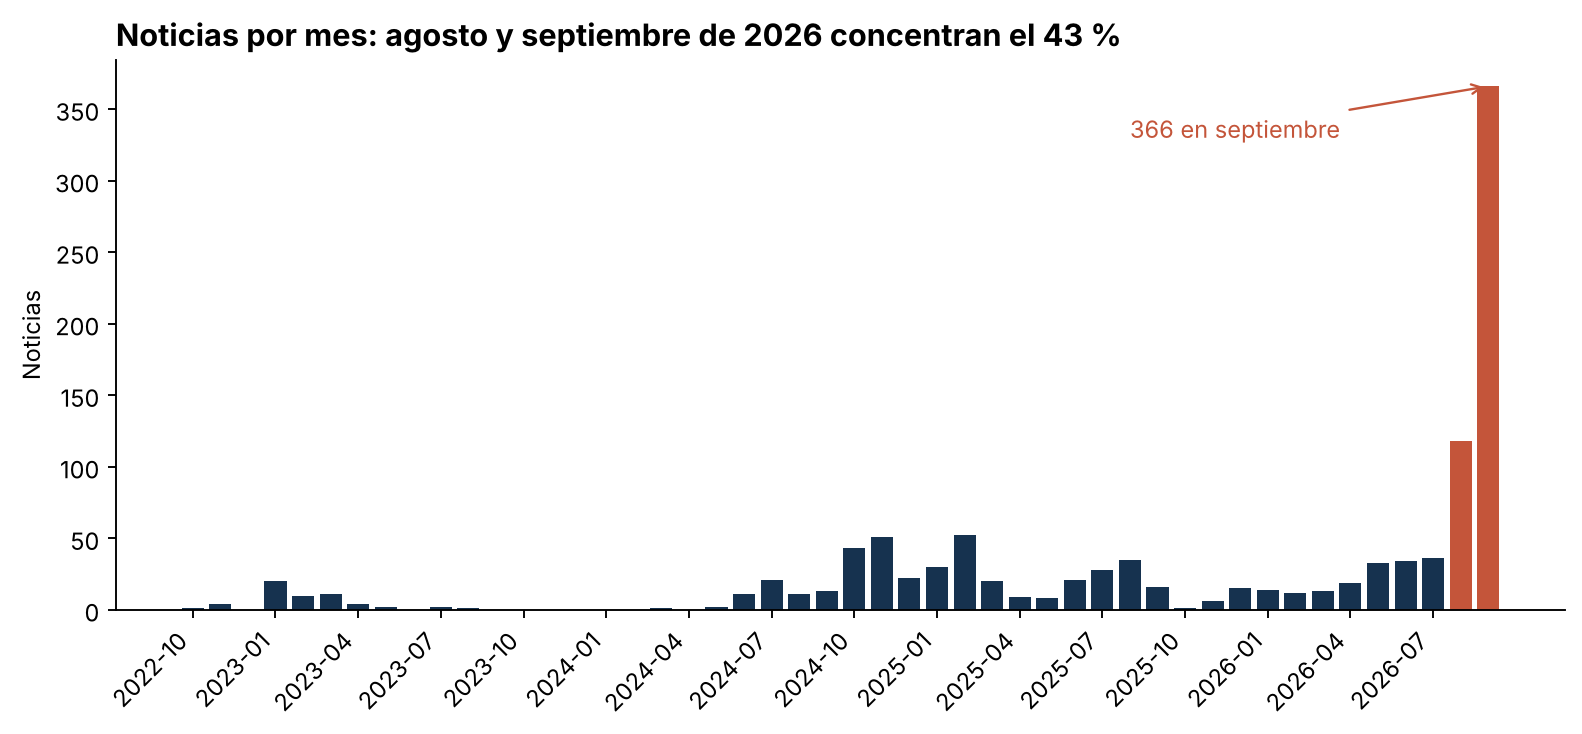
\includegraphics[width=0.95\textwidth]{figures/02_noticias_por_mes.png}
\caption{Noticias por mes.}
\label{fig:mes}
\end{figure}
Septiembre de 2026 reúne 366 noticias y, junto con agosto, el 43,4\,\% del total (484 de 1\,116). Ningún mes anterior pasa de 52 noticias, y 21 de los 48 meses del periodo tienen menos de 10. Cualquier conclusión sobre horas o días queda dominada por esas siete semanas.

\begin{figure}[H]\centering
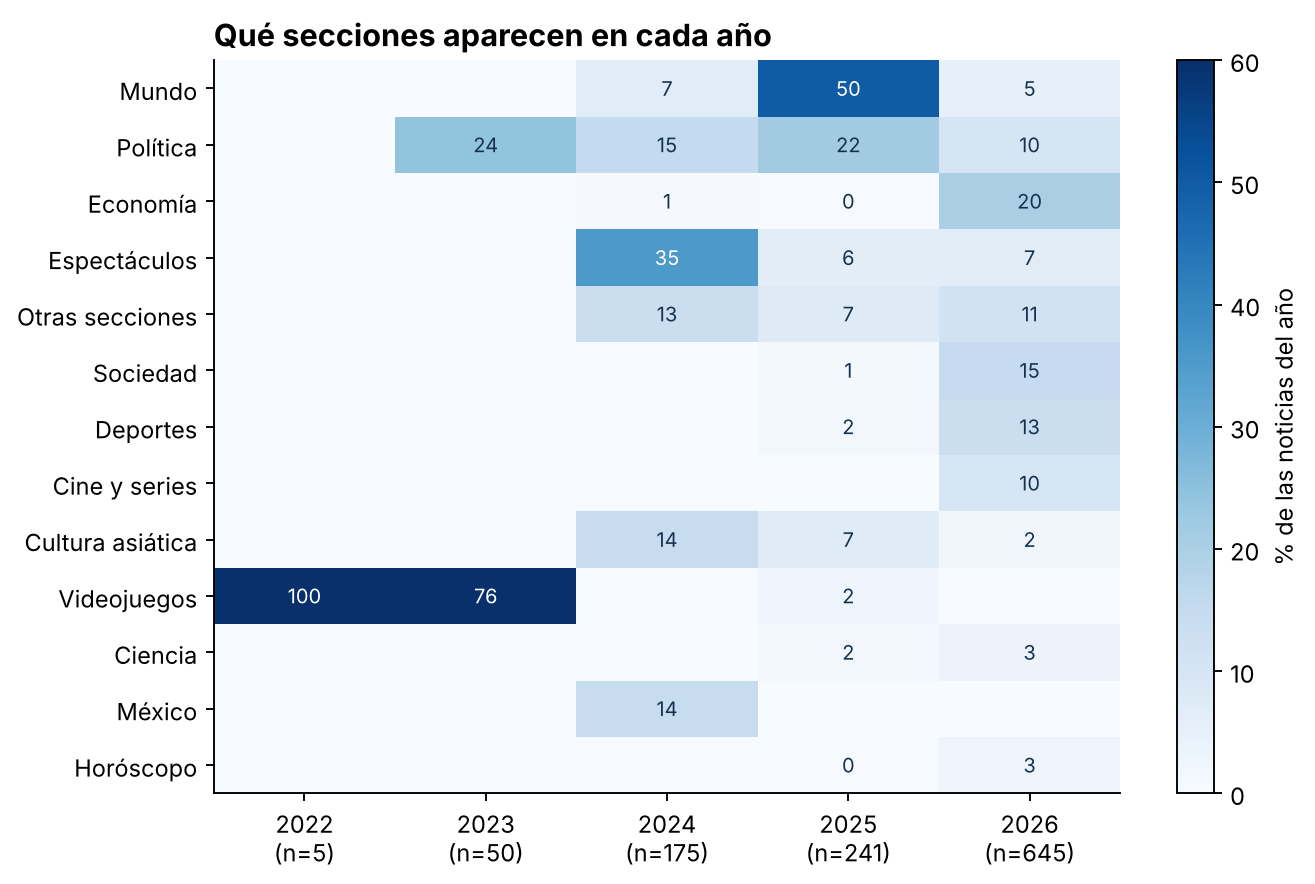
\includegraphics[width=0.82\textwidth]{figures/03_seccion_por_anio.png}
\caption{Peso de cada sección dentro de cada año (\%).}
\label{fig:seccion-anio}
\end{figure}
La relación entre sección y año es fuerte ($\chi^2 = 1\,506$; V de Cramér = 0,61; $p < 0{,}001$). Videojuegos es casi todo de 2022-2023 (43 de 49 noticias), México aparece solo en 2024, Mundo es la mitad de 2025 y 131 de las 133 notas de Economía son de 2026. La composición por sección refleja el calendario del scraping y no el peso editorial real. El 40\,\% de las celdas tiene frecuencia esperada menor que 5, así que el valor exacto de $V$ es aproximado, pero el patrón es evidente.

\subsection{Anomalías en hora y fecha}
\begin{figure}[H]\centering
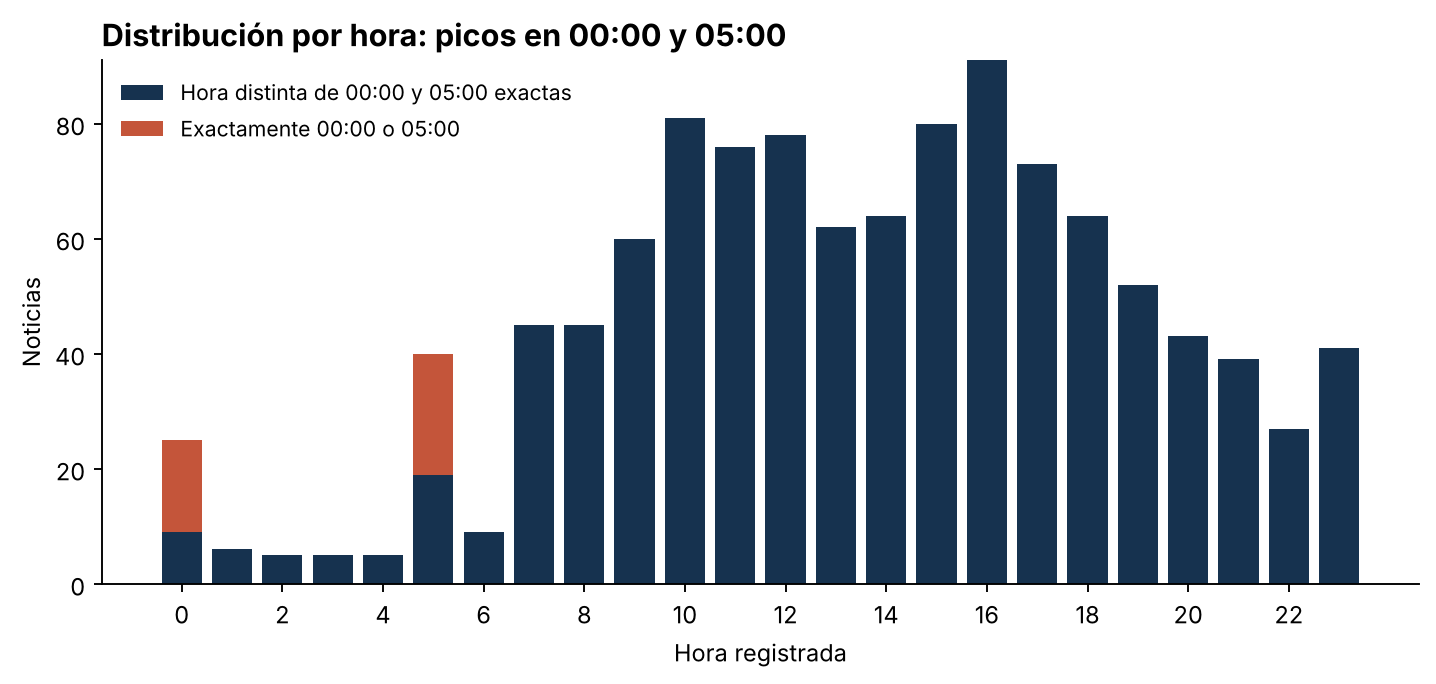
\includegraphics[width=0.88\textwidth]{figures/04_horas.png}
\caption{Noticias por hora registrada.}
\label{fig:horas}
\end{figure}
Hay 37 noticias (3,3\,\%) exactamente a las 00:00 o a las 05:00, cuando cada hora entre la 01 y las 04 tiene unas 5. Trece de las 16 de medianoche son horóscopos programados. Si se excluyen, la madrugada baja de 7,7\,\% a 4,5\,\%.

\begin{figure}[H]\centering
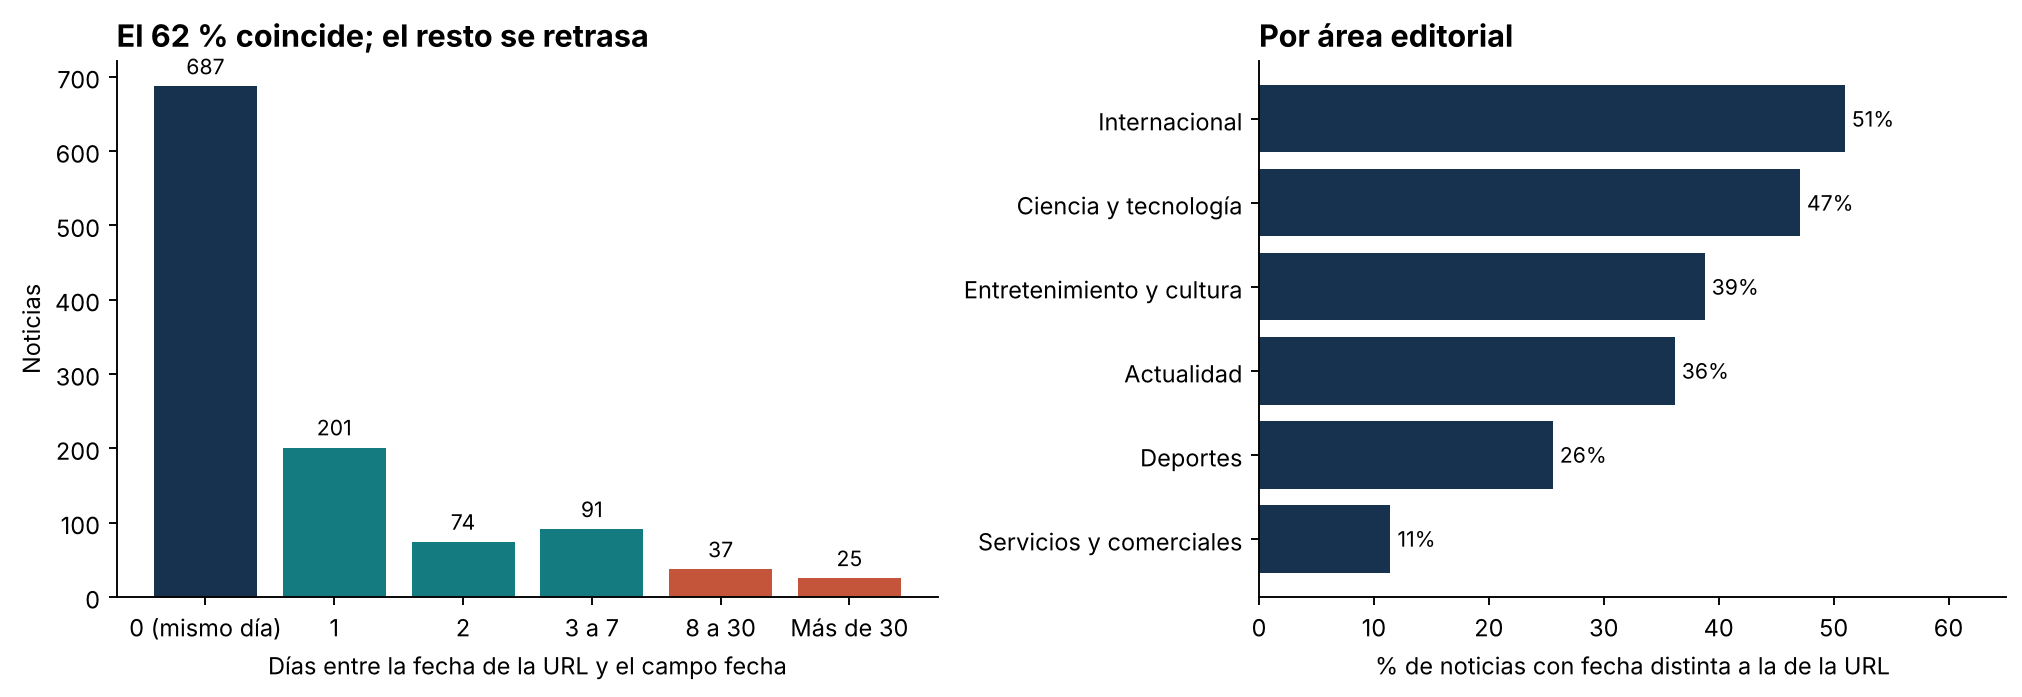
\includegraphics[width=\textwidth]{figures/05_desfase_fechas.png}
\caption{Diferencia entre la fecha de la URL y el campo \texttt{fecha}.}
\label{fig:desfase}
\end{figure}
De las 1\,115 noticias con fecha en la URL, el 61,6\,\% coincide con \texttt{fecha} y el 38,4\,\% no. \textbf{Nunca hay desfases negativos}: \texttt{fecha} es siempre igual o posterior. La mayoría de las diferencias es pequeña (el 90\,\% está por debajo de 4 días), pero hay 25 noticias con más de 30 días y casos extremos, como una nota de «Datos LR» con URL de diciembre de 2021 y fecha de mayo de 2026 (1\,632 días). La hipótesis de zona horaria no se sostiene: el desfase de 1 día no se concentra en la noche (15\,\% de las noticias de 19\,h en adelante frente a 20\,\% entre las de mismo día).

Lo más consistente es que \texttt{fecha} sea a veces la fecha de \textbf{actualización o republicación visible en la página}, no la de publicación original. Esto no se puede confirmar con los datos disponibles. El desfase varía entre áreas ($\chi^2 = 32{,}9$; $V = 0{,}17$, efecto pequeño): Internacional tiene la mayor proporción (51\,\%) y Servicios y comerciales la menor (11\,\%).

\subsection{Autores y etiquetas}
\label{sec:autores}
\begin{figure}[H]\centering
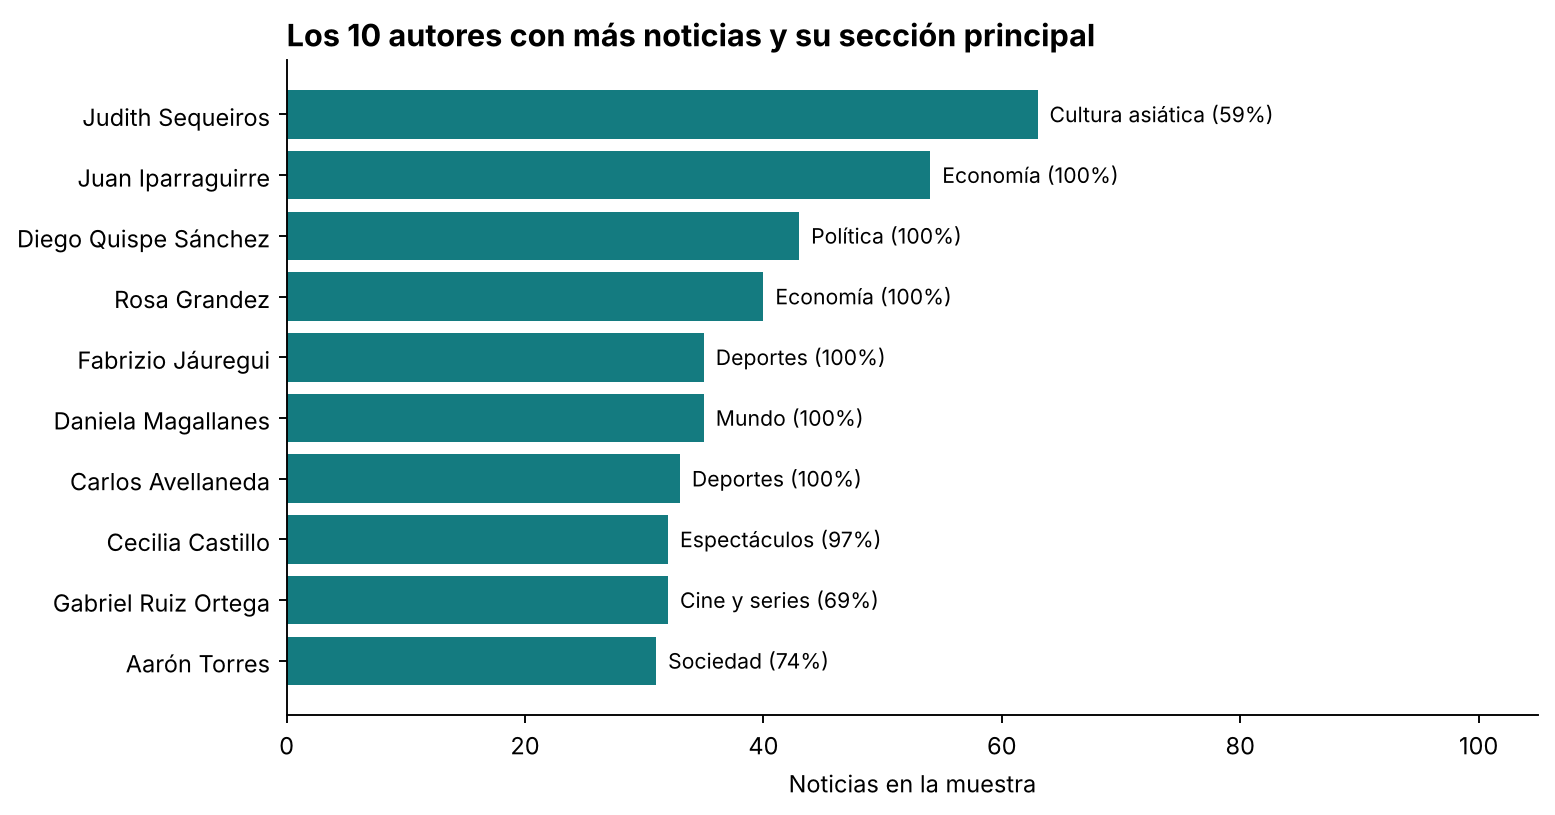
\includegraphics[width=0.85\textwidth]{figures/06_autores_especializacion.png}
\caption{Los 10 autores con más noticias y su sección principal.}
\label{fig:autores}
\end{figure}
Los diez primeros autores suman el 35,66\,\% de la muestra. Siete de ellos tienen al menos el 97\,\% de sus notas en una sola sección y seis el 100\,\% (Iparraguirre y Grandez en Economía, Quispe en Política, Magallanes en Mundo, Jáuregui y Avellaneda en Deportes). Judith Sequeiros, la más frecuente (63), tiene el 59\,\% en Cultura asiática. El autor es casi un proxy de la sección, y no aporta información independiente. Además, 25 notas (2,2\,\%) tienen firma institucional.

\begin{figure}[H]\centering
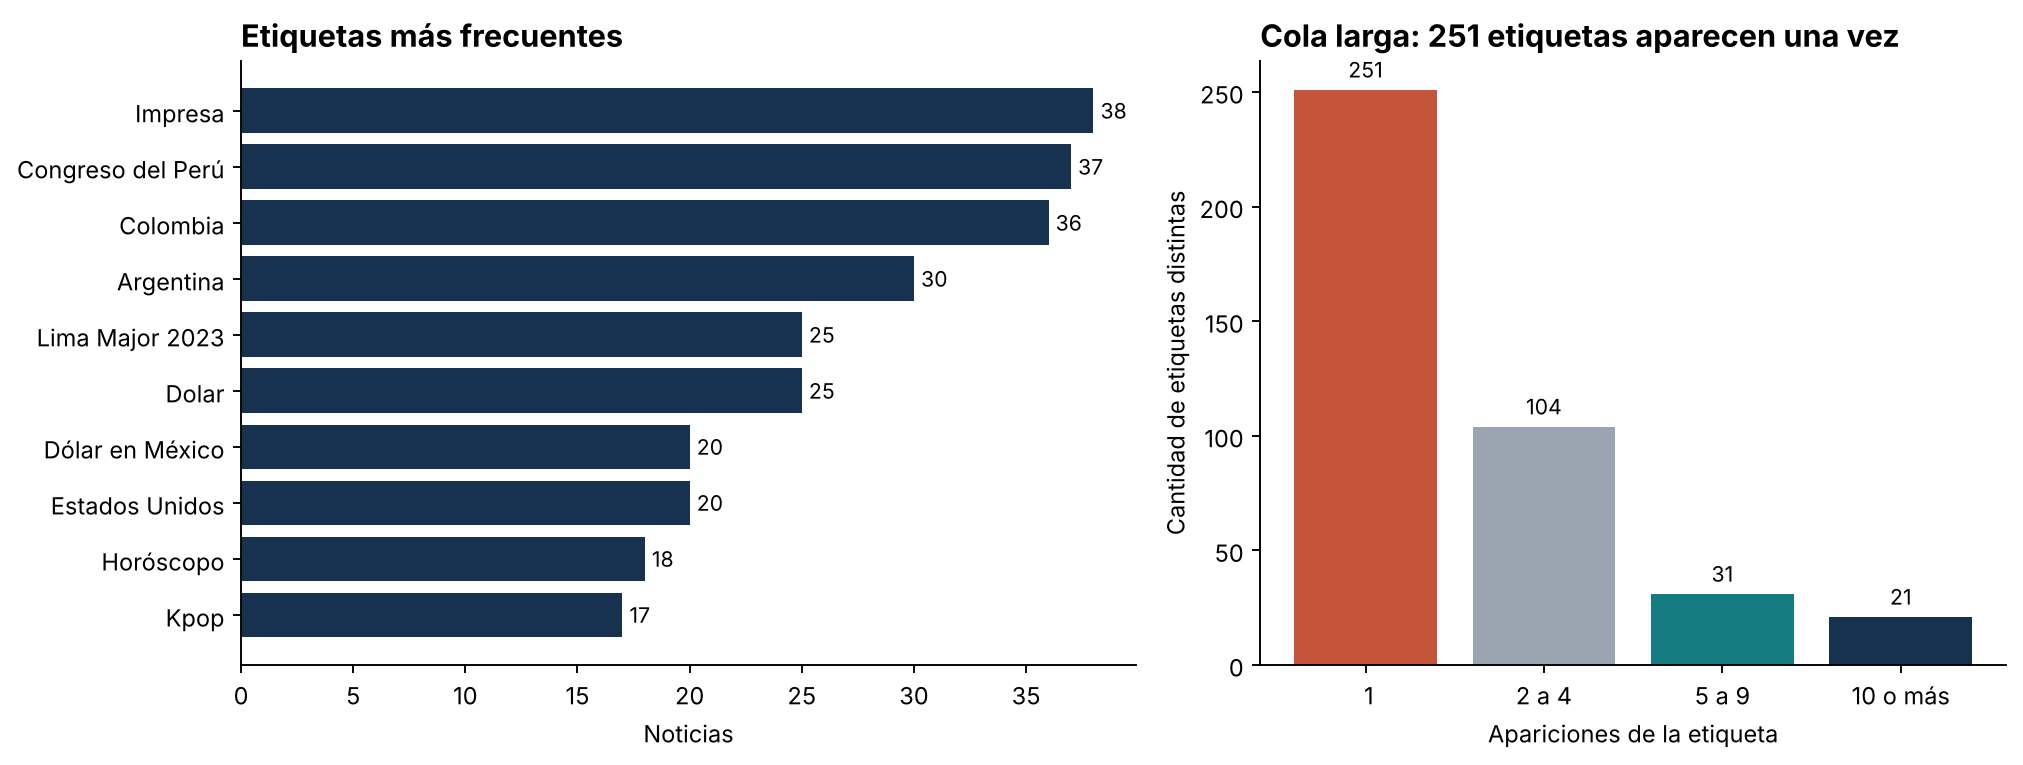
\includegraphics[width=0.95\textwidth]{figures/07_etiquetas.png}
\caption{Etiquetas más frecuentes y cola larga.}
\label{fig:etiquetas}
\end{figure}
Hay 408 etiquetas y 251 aparecen una vez. Solo 52 tienen 5 o más apariciones (sin contar «Sin etiqueta») y cubren el 53\,\% de las filas. La más frecuente, Impresa, llega a 38 noticias (3,4\,\%). Las etiquetas sirven para buscar temas puntuales (Congreso del Perú, Colombia, Dólar) pero no para comparar grupos, por eso las comparaciones usan \texttt{seccion} y \texttt{area\_editorial}.

\subsection{Titulares}
\begin{figure}[H]\centering
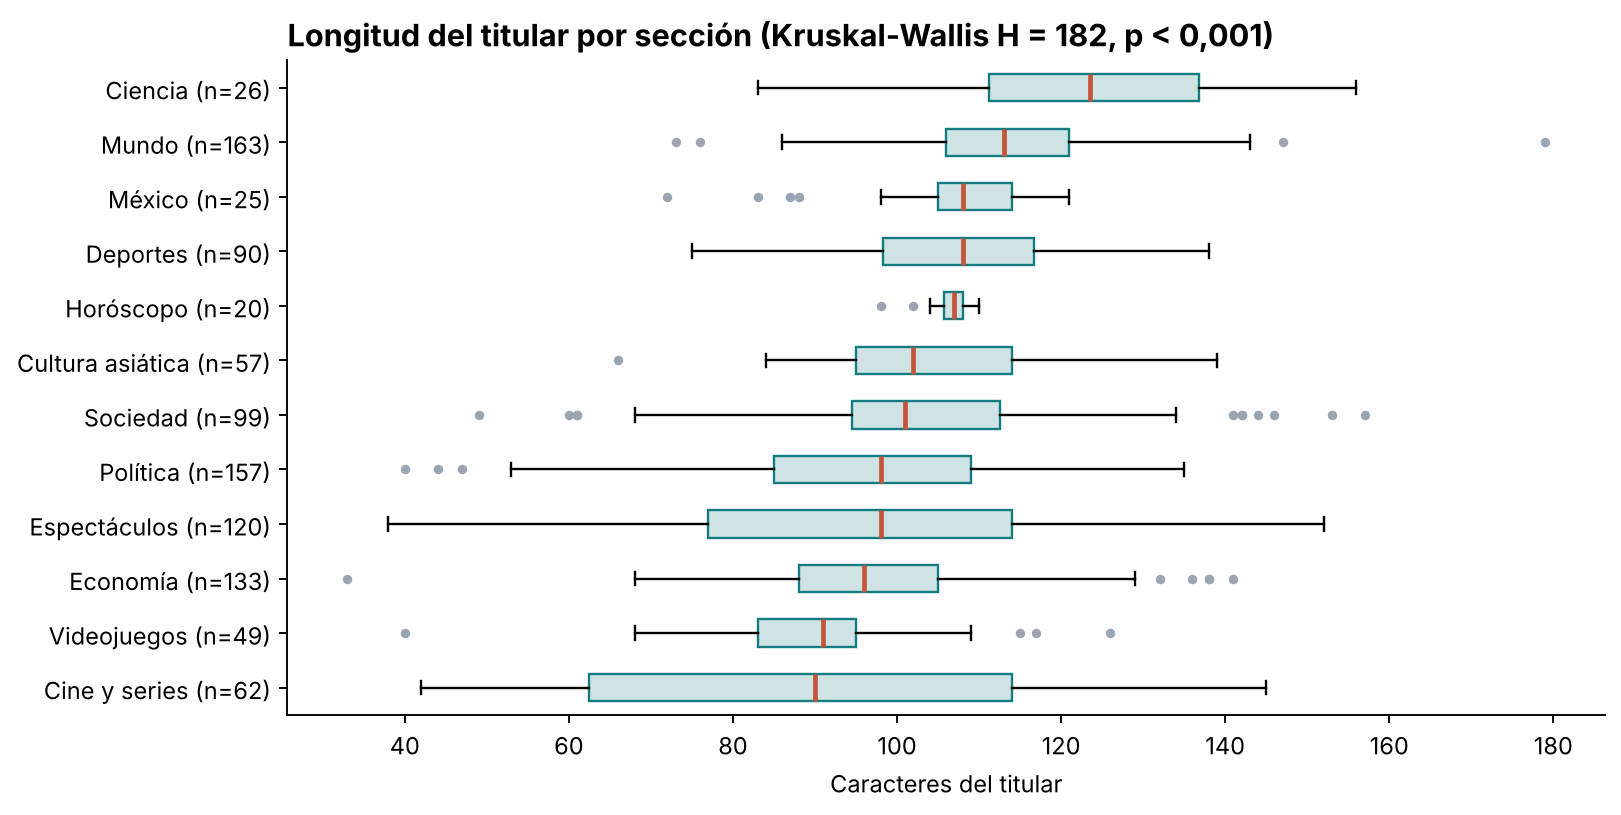
\includegraphics[width=0.88\textwidth]{figures/09_longitud_por_seccion.png}
\caption{Longitud del titular por sección.}
\label{fig:longitud}
\end{figure}
La mediana global es de 103 caracteres (rango de 33 a 191). Se usó Kruskal-Wallis porque la longitud no cumple los supuestos de ANOVA entre grupos. Hay diferencias entre secciones ($H = 182{,}3$; $p < 0{,}001$; $\varepsilon^2 = 0{,}18$, efecto mediano): Ciencia tiene los titulares más largos (mediana 124) y Cine y series los más cortos (90).

\begin{figure}[H]\centering
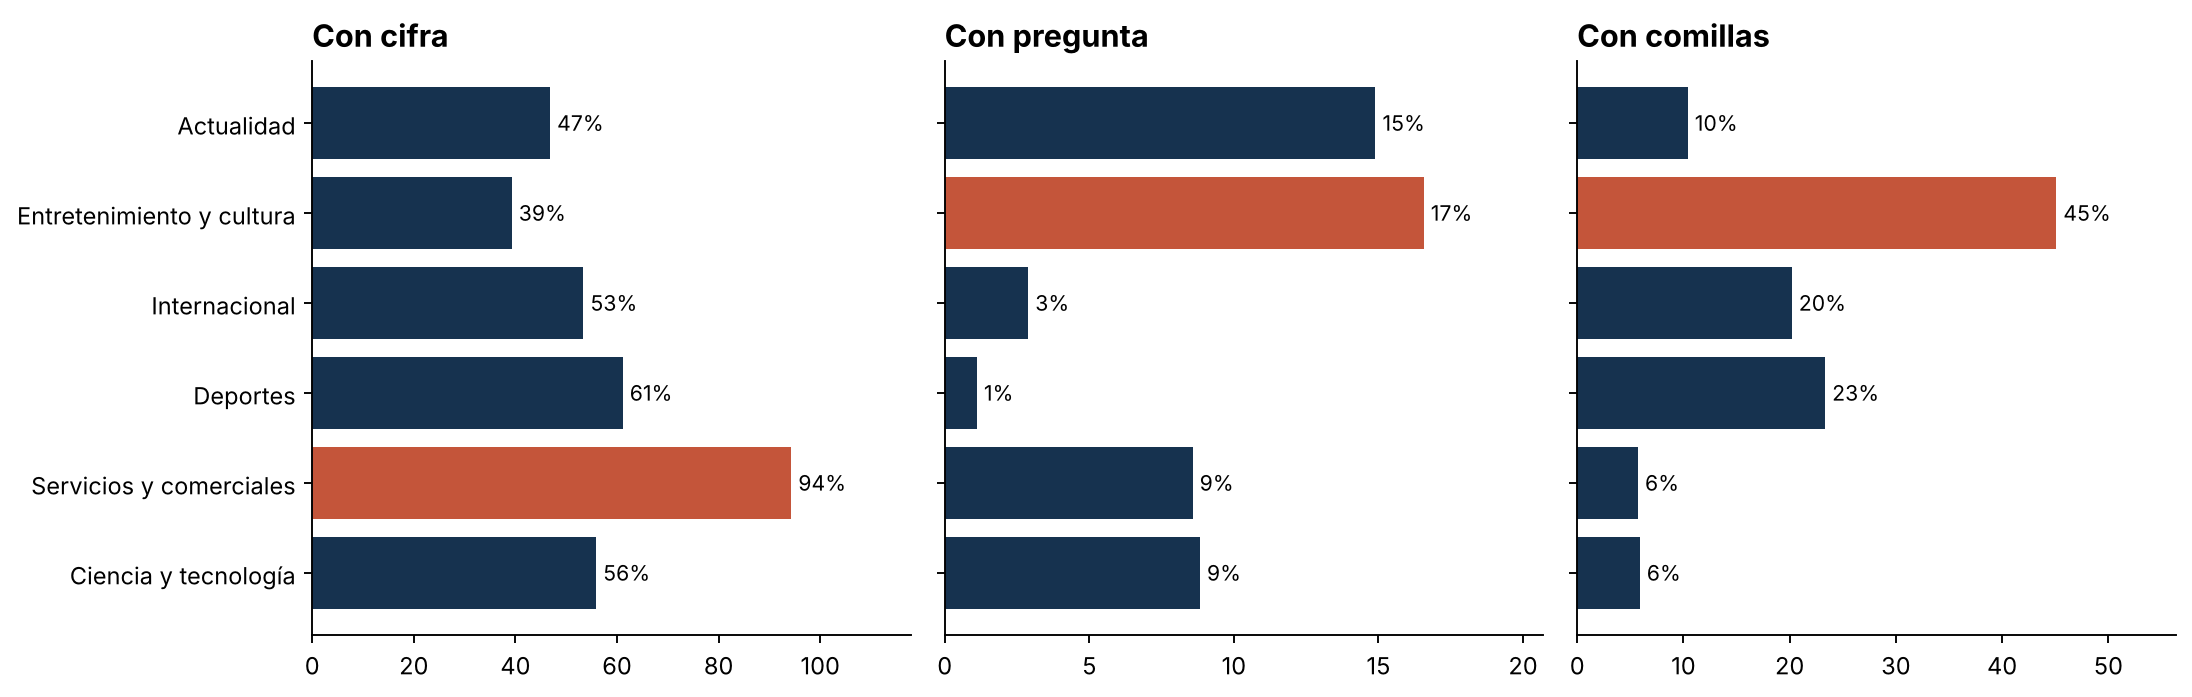
\includegraphics[width=\textwidth]{figures/10_rasgos_titular_area.png}
\caption{Porcentaje de titulares con cifra, pregunta y comillas por área editorial.}
\label{fig:rasgos}
\end{figure}
Los tres rasgos dependen del área (las tres pruebas dan $p < 0{,}001$). Las \textbf{comillas} muestran el efecto más grande ($V = 0{,}35$): Entretenimiento y cultura cita declaraciones en el 45\,\% de sus titulares frente al 10\,\% de Actualidad. Las \textbf{cifras} aparecen en el 94\,\% de los titulares de Servicios y comerciales (horóscopos y loterías) y en el 61\,\% de Deportes, y en solo el 39\,\% de Entretenimiento. Las \textbf{preguntas} son frecuentes en Entretenimiento (17\,\%) y Actualidad (15\,\%), y casi no existen en Deportes (1\,\%) ni en Internacional (3\,\%). Son diferencias de estilo de redacción; la muestra no permite decir nada sobre audiencia.

\subsection{Horarios, días y formato de URL}
\begin{figure}[H]\centering
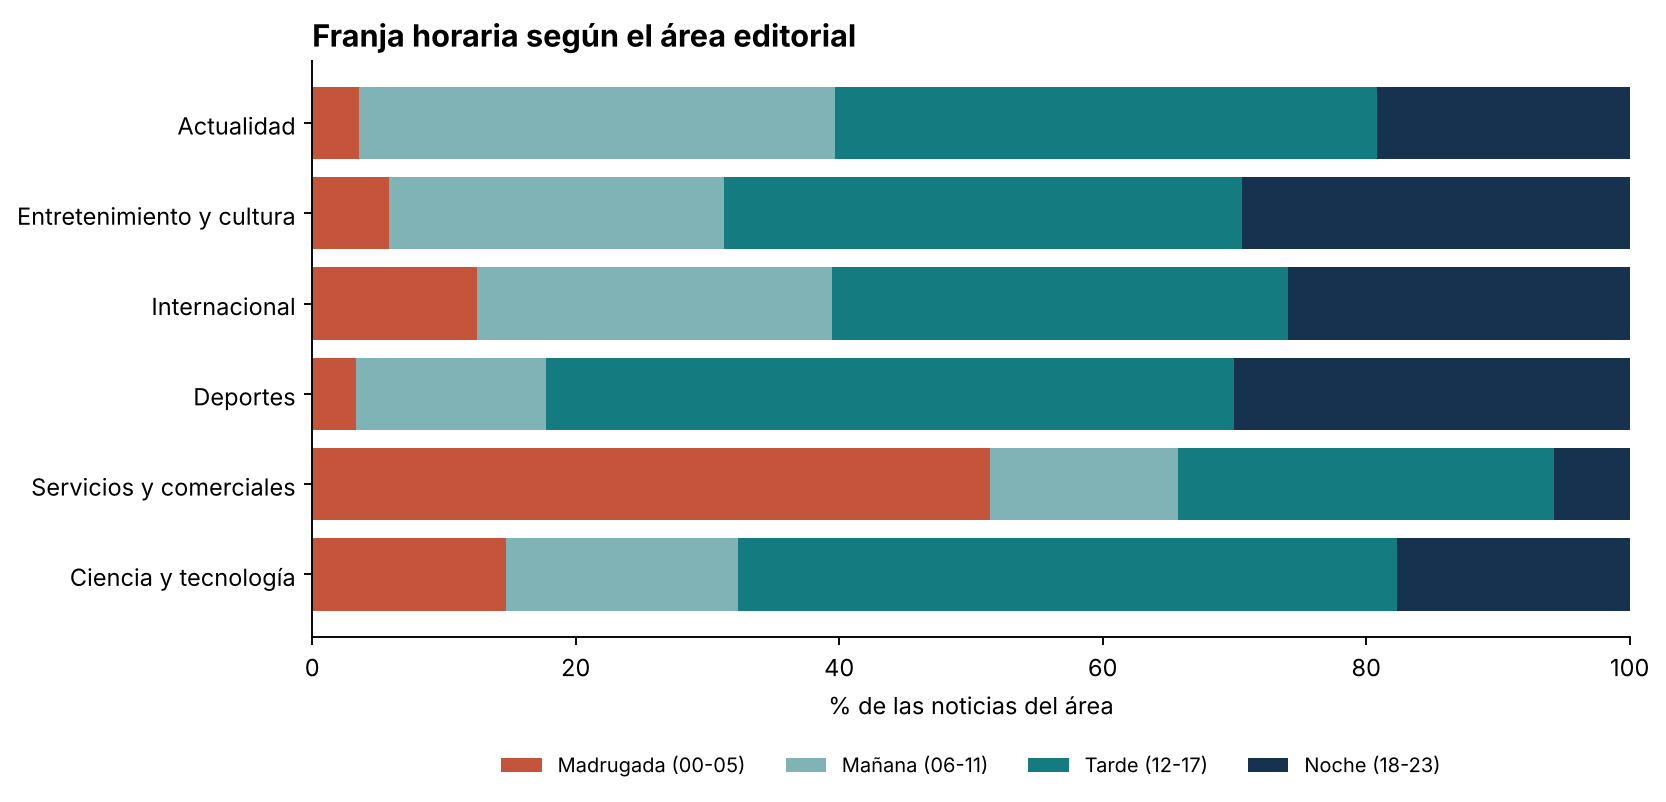
\includegraphics[width=0.88\textwidth]{figures/11_franja_por_area.png}
\caption{Franja horaria por área editorial.}
\label{fig:franja}
\end{figure}
La tarde (12:00 a 17:59) reúne 448 noticias (40,1\,\%). El horario depende del área ($\chi^2 = 151$; $V = 0{,}21$; $p < 0{,}001$): Servicios y comerciales publica el 51\,\% en madrugada (contenido programado), mientras que Deportes y Ciencia y tecnología tienen la mitad de sus notas por la tarde.

\begin{figure}[H]\centering
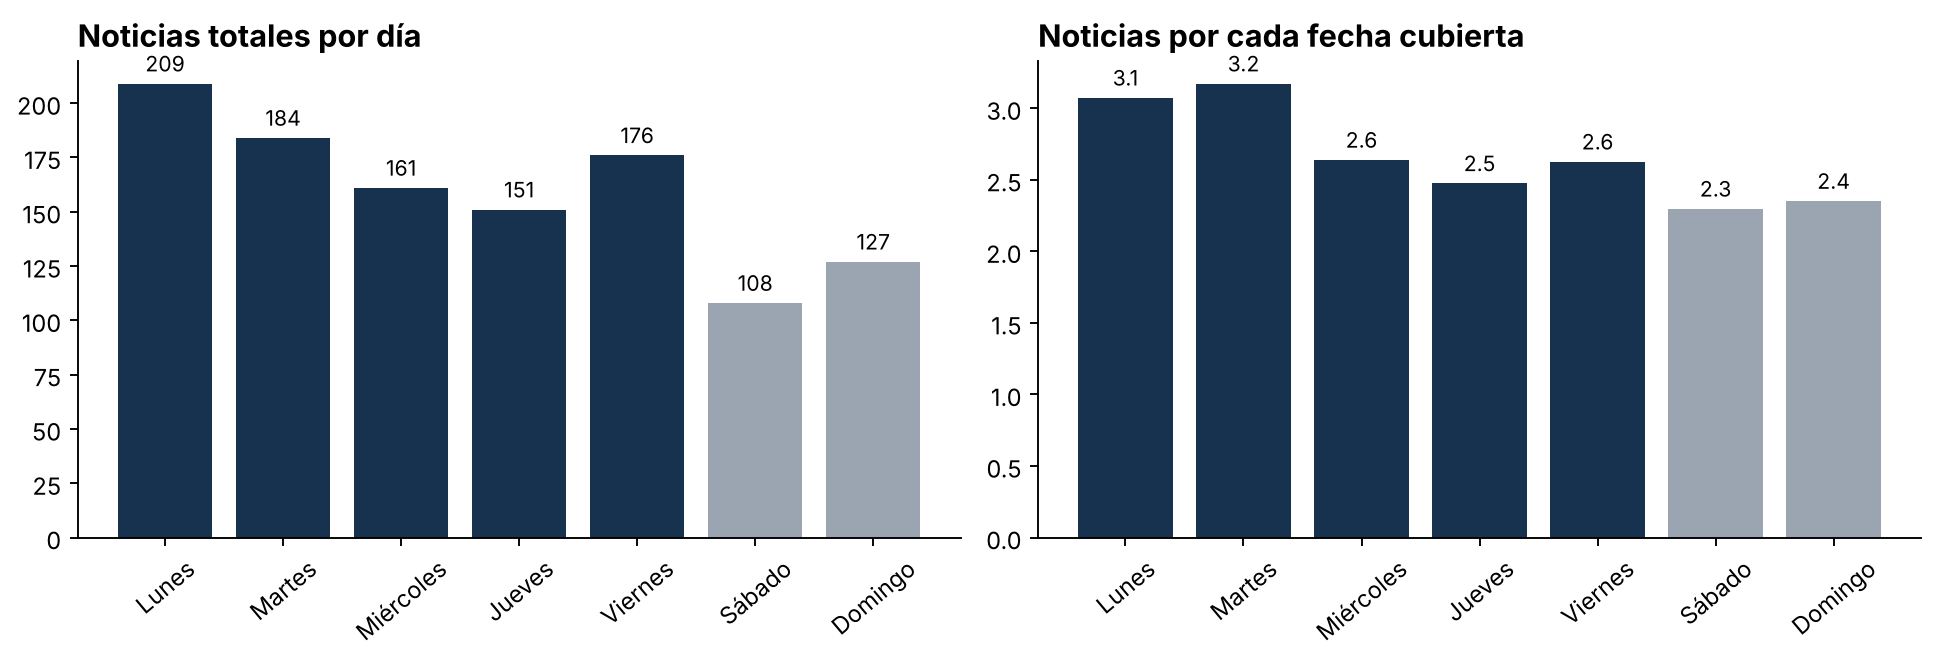
\includegraphics[width=0.97\textwidth]{figures/12_dias_semana.png}
\caption{Noticias por día de la semana, totales y por fecha cubierta.}
\label{fig:dias}
\end{figure}
Hay 209 noticias en lunes y 108 en sábado, pero la diferencia viene sobre todo de cuántas fechas se cubrieron: 68 lunes frente a 47 sábados. Al dividir por fecha cubierta, la brecha se reduce a 3,1 frente a 2,3 noticias. Entre semana hay algo más de noticias por fecha, pero esto depende del scraping.

\begin{figure}[H]\centering
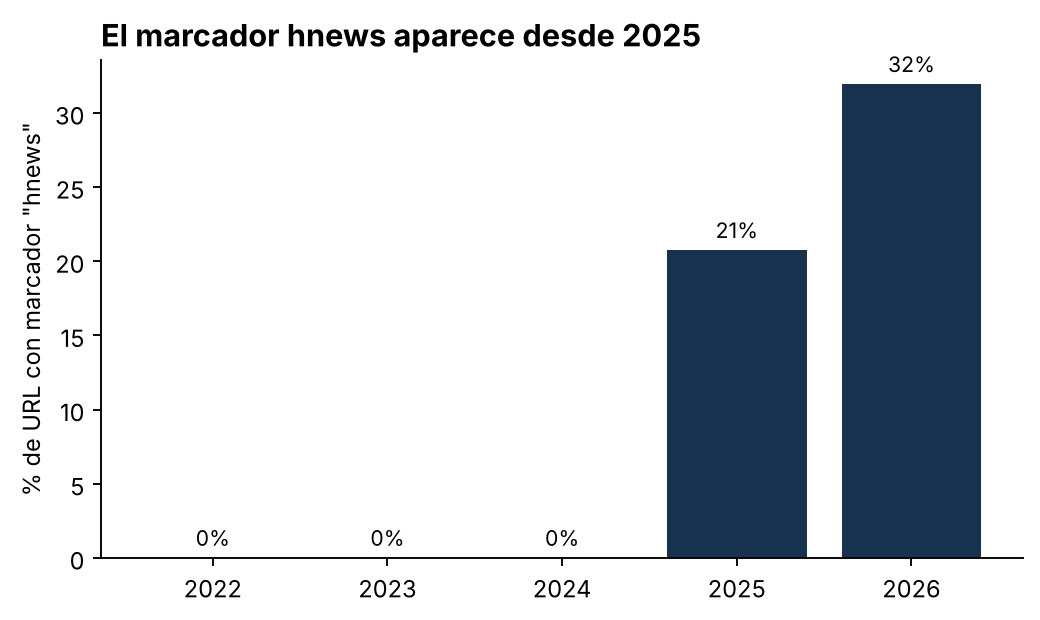
\includegraphics[width=0.68\textwidth]{figures/13_url_hnews_anio.png}
\caption{Porcentaje de URL con el marcador \texttt{hnews} por año.}
\label{fig:hnews}
\end{figure}
Ninguna URL de 2022 a 2024 tiene el marcador \texttt{hnews}; aparece en el 21\,\% de 2025 y el 32\,\% de 2026 ($V = 0{,}30$). Indica un cambio en el formato de URL y no una categoría editorial. Las URL con \texttt{hnews} tienen más desfases (53\,\% frente a 34\,\%), por lo que conviene no mezclarlas sin revisar.

\subsection{Resumen de pruebas estadísticas}
\begin{table}[H]\centering
\caption{Pruebas estadísticas, ordenadas por tamaño de efecto.}
\begin{tabular}{p{4.6cm}p{3.1cm}p{2.2cm}p{1.6cm}p{1.8cm}}
\toprule
\textbf{Relación} & \textbf{Prueba} & \textbf{Estadístico} & \textbf{$p$} & \textbf{Efecto}\\\midrule
Sección × año & $\chi^2$ (gl = 44) & 1\,505,6 & $<$\,0,001 & $V = 0{,}61$\\
Titular con comillas × área & $\chi^2$ (gl = 5) & 139,7 & $<$\,0,001 & $V = 0{,}35$\\
Formato \texttt{hnews} × año & $\chi^2$ (gl = 4) & 98,7 & $<$\,0,001 & $V = 0{,}30$\\
Franja horaria × área & $\chi^2$ (gl = 15) & 151,0 & $<$\,0,001 & $V = 0{,}21$\\
Titular con cifra × área & $\chi^2$ (gl = 5) & 49,4 & $<$\,0,001 & $V = 0{,}21$\\
Titular con pregunta × área & $\chi^2$ (gl = 5) & 37,8 & $<$\,0,001 & $V = 0{,}18$\\
Desfase de fecha × área & $\chi^2$ (gl = 5) & 32,9 & $<$\,0,001 & $V = 0{,}17$\\
Longitud del titular $\sim$ sección & Kruskal-Wallis (gl = 11) & 182,3 & $<$\,0,001 & $\varepsilon^2 = 0{,}18$\\
\bottomrule
\end{tabular}
\end{table}

% =====================================================================
\section{Insights encontrados}
Los usuarios que tenemos en mente son dos: (a) quien quiera \textbf{reutilizar esta colección} para un análisis posterior, y (b) una redacción o analista de medios interesado en el \textbf{perfil editorial} de las secciones. Las recomendaciones se dirigen a ellos.

{\small
\begin{longtable}{p{5.0cm}p{6.2cm}p{3.3cm}}
\caption{Hallazgos, recomendaciones y beneficiarios.}\\
\toprule
\textbf{Hallazgo y evidencia} & \textbf{Qué hacer} & \textbf{Quién se beneficia}\\\midrule
\endfirsthead
\toprule
\textbf{Hallazgo y evidencia} & \textbf{Qué hacer} & \textbf{Quién se beneficia}\\\midrule
\endhead
El 43,4\,\% de las noticias es de ago-sep 2026 y sección × año tiene $V = 0{,}61$ & Al recolectar de nuevo, fijar una cuota por mes y por sección. Mientras tanto, no medir el peso de una sección con esta colección & Quien amplíe el dataset\\
\texttt{fecha} $\ge$ fecha de la URL siempre; 38,4\,\% difiere y hay 25 casos de más de 30 días & Validar la fecha en el HTML (publicación o actualización) antes de modelar series de tiempo; si se necesita la original, usar \texttt{fecha\_url} & Quien analice tendencias\\
37 noticias a las 00:00 y 05:00 exactas; 51\,\% de Servicios y comerciales en madrugada & Excluir \texttt{hora\_sospechosa} y Servicios al estudiar horarios de una redacción & Quien estudie horarios\\
6 de los 10 autores principales publican 100\,\% en una sola sección & Para comparar redacciones, usar sección o área, no autor. Para productividad individual hace falta un muestreo por fecha & Analista de medios\\
251 de 408 etiquetas aparecen una vez; 52 cubren el 53\,\% de las filas & Usar \texttt{tag\_agrupado} para comparar y la etiqueta original solo para buscar temas & Quien trabaje con temas\\
Comillas: 45\,\% en Entretenimiento frente a 10\,\% en Actualidad ($V = 0{,}35$); longitud: $\varepsilon^2 = 0{,}18$ & Usar estos perfiles como línea base de estilo por área, y revisar desvíos al editar & Redacción\\
\texttt{hnews} aparece solo desde 2025 y se asocia a más desfases & Tratarlo como marca del formato de URL y separarlo al analizar fechas & Quien procese las URL\\
\bottomrule
\end{longtable}
}

% =====================================================================
\section{Conclusiones}
\textbf{Sobre los objetivos.}
\begin{enumerate}
\item El sesgo temporal se midió: el 43,4\,\% de la colección es de agosto y septiembre de 2026 y la composición por sección cambia fuertemente con el año, así que no sirve para estimar el peso editorial de una sección.
\item La fecha es la variable menos confiable: nunca es anterior a la de la URL, difiere en el 38,4\,\% de los casos y puede ser fecha de actualización; la hora tiene 37 valores atípicos probablemente programados.
\item El autor es casi equivalente a la sección y las etiquetas están muy dispersas, por lo que ambas sirven más para explorar que para comparar.
\item El estilo del titular y el horario sí cambian entre áreas editoriales, con efectos moderados ($V$ entre 0,17 y 0,35).
\item Se entrega un dataset documentado de 31 variables y un pipeline que se ejecuta con un comando.
\end{enumerate}

\textbf{Reflexión crítica y límites.} Los resultados describen esta colección y no el diario. Los valores $p$ no se pueden generalizar porque no hay muestreo aleatorio. El catálogo de áreas editoriales es criterio del grupo y otra agrupación podría matizar algunas comparaciones. No se dispone de texto ni de métricas de lectura, por lo que no se puede hablar de interés de los lectores ni de calidad.

\textbf{Trabajo futuro.} Recolectar por ventanas de fechas con cuotas por sección; capturar en el scraping la fecha de publicación y la de última actualización por separado; y, si se obtiene el cuerpo de las notas, analizar su contenido y no solo el titular.

% =====================================================================
\section{Documentación y reproducibilidad en GitHub}
\textbf{Repositorio} \cite{repo}:\\
\url{https://github.com/josueTori-UTEC/ACD-Analisis-Noticias-LaRepublica}

\begin{table}[H]\centering
\caption{Estructura del repositorio.}
\begin{tabular}{p{4.6cm}p{10cm}}
\toprule
\textbf{Ruta} & \textbf{Contenido}\\\midrule
\texttt{README.md}, \texttt{requirements.txt} & Descripción, instrucciones y dependencias\\
\texttt{run\_all.py} & Ejecuta el pipeline completo (notebooks 01 y 02)\\
\texttt{data/} & CSV original, CSV final y base SQLite\\
\texttt{notebooks/} & \texttt{01\_preprocesamiento.ipynb} y \texttt{02\_analisis\_visualizacion.ipynb}, con salidas guardadas\\
\texttt{docs/} & Diccionarios de datos inicial y final (PDF y DOCX)\\
\texttt{results/}, \texttt{figures/} & Indicadores, resúmenes, pruebas estadísticas y 14 gráficos\\
\texttt{reports/}, \texttt{presentacion/} & Informe en PDF y DOCX; presentación en PPTX y PDF; guion de exposición\\
\bottomrule
\end{tabular}
\end{table}

\textbf{Cómo reproducir.} Requiere Python 3.10 o posterior. Desde la raíz del repositorio:
\begin{lstlisting}
pip install -r requirements.txt
python run_all.py
\end{lstlisting}
El comando lee el CSV original, regenera el CSV final, la base SQLite, los resultados y los 14 gráficos. También se pueden abrir los notebooks en Jupyter y ejecutarlos en orden (01 y luego 02). No se necesita conexión a internet.

\textbf{Historial:} cada etapa de la Parte II se subió en commits separados y con mensajes descriptivos (preprocesamiento, análisis, diccionario, informe y presentación), de modo que el historial refleja la evolución del trabajo.

\begin{thebibliography}{99}
\bibitem{larepublica} La República. \textit{Portal de noticias}. \url{https://larepublica.pe}
\bibitem{repo} Grupo 3, DS3021. \textit{ACD-Analisis-Noticias-LaRepublica}. Repositorio del proyecto. \url{https://github.com/josueTori-UTEC/ACD-Analisis-Noticias-LaRepublica}
\end{thebibliography}

\end{document}
